\documentclass{sbc2023}

% Standard Packages from Template
\usepackage{graphicx}
\usepackage[misc,geometry]{ifsym} 
\usepackage{fontspec}
\usepackage{fontawesome}
\usepackage{academicons}
\usepackage{color}
\usepackage{hyperref} 
\usepackage{aas_macros}
\usepackage[bottom]{footmisc}
\usepackage{supertabular}
\usepackage{afterpage}
\usepackage{url}
\usepackage{pifont}
\usepackage{multicol}
\usepackage{multirow}
\usepackage{tabularx}
\usepackage{ragged2e}
% Additional Packages imported from user's main.tex for compatibility
\usepackage{booktabs}
\usepackage{listings}
\usepackage{xcolor}
\usepackage{amsmath}
\usepackage{amssymb}
\usepackage{subcaption}
\usepackage{tabularx}
\usepackage{calc}
\usepackage{tikz}
\usepackage{algorithm}
\usepackage{algpseudocode}
\usepackage{rotating}
\usepackage{float}
\usepackage{comment}

% TikZ library for drawing figures (CORRECTED)
\usetikzlibrary{shapes, arrows.meta, positioning}

% Citation style as per template
\setcitestyle{square}

% Color definitions from user's main.tex
\definecolor{orcidlogo}{rgb}{0.37,0.48,0.13}
\definecolor{unilogo}{rgb}{0.16, 0.26, 0.58}
\definecolor{maillogo}{rgb}{0.58, 0.16, 0.26}
\definecolor{darkblue}{rgb}{0.0,0.0,0.0}
\hypersetup{colorlinks,breaklinks,
            linkcolor=darkblue,urlcolor=darkblue,
            anchorcolor=darkblue,citecolor=darkblue}

\definecolor{codegreen}{rgb}{0,0.6,0}
\definecolor{codegray}{rgb}{0.5,0.5,0.5}
\definecolor{codepurple}{rgb}{0.58,0,0.82}
\definecolor{backcolour}{rgb}{0.95,0.95,0.92}

% Listings style from user's main.tex
\lstdefinestyle{mystyle}{
    backgroundcolor=\color{backcolour},
    commentstyle=\color{codegreen},
    keywordstyle=\color{magenta},
    numberstyle=\tiny\color{codegray},
    stringstyle=\color{codepurple},
    basicstyle=\ttfamily\footnotesize,
    breakatwhitespace=false,
    breaklines=true,
    captionpos=b,
    keepspaces=true,
    numbers=left,
    numbersep=5pt,
    showspaces=false,
    showstringspaces=false,
    showtabs=false,
    tabsize=2,
    inputencoding=utf8,
    extendedchars=true,
    literate={á}{{\'a}}1 {é}{{\'e}}1 {í}{{\'i}}1 {ó}{{\'o}}1 {ú}{{\'u}}1 {Á}{{\'A}}1 {É}{{\'E}}1 {Í}{{\'I}}1 {Ó}{{\'O}}1 {Ú}{{\'U}}1 {à}{{\`a}}1 {è}{{\`e}}1 {ì}{{\`i}}1 {ò}{{\`o}}1 {ù}{{\`u}}1 {À}{{\`A}}1 {È}{{\`E}}1 {Ì}{{\`I}}1 {Ò}{{\`O}}1 {Ù}{{\'U}}1 {ä}{{\"a}}1 {ë}{{\"e}}1 {ï}{{\"i}}1 {ö}{{\"o}}1 {ü}{{\"u}}1 {Ä}{{\"A}}1 {Ë}{{\"E}}1 {Ï}{{\"I}}1 {Ö}{{\"O}}1 {Ü}{{\"U}}1 {â}{{\^a}}1 {ê}{{\^e}}1 {î}{{\^i}}1 {ô}{{\^o}}1 {û}{{\^u}}1 {Â}{{\^A}}1 {Ê}{{\^E}}1 {Î}{{\^I}}1 {Ô}{{\^O}}1 {Û}{{\^U}}1 {ç}{{\c{c}}}1 {Ç}{{\c{C}}}1 {ã}{{\~a}}1 {õ}{{\~o}}1 {Ã}{{\~A}}1 {Õ}{{\~O}}1 {ñ}{{\~n}}1 {Ñ}{{\~N}}1
}
\lstset{style=mystyle}

\jid{JBCS}
\jtitle{Journal of the Brazilian Computer Society, 2025, XX:1, }
\doi{10.5753/jbcs.2025.XXXXXX}
\copyrightstatement{This work is licensed under a Creative Commons Attribution 4.0 International License}
\jyear{2025}

\title[Driver Assistance System Based on YOLO Object Detection]{A Driver Assistance System Based on YOLO Object Detection: Development and Experimental Validation in the CARLA Simulator}

\author[Gomes \& Tamariz 2025]{
\affil{\textbf{Daniel Terra Gomes}~\href{https://orcid.org/0009-0003-0701-5889}{\textcolor{orcidlogo}{\aiOrcid}}~\textnormal{\textcolor{blue}{\faEnvelopeO}}~~[~\textbf{Universidade Estadual do Norte Fluminense Darcy Ribeiro}~|\href{mailto:danielterra@pq.uenf.br}{~\textbf{danielterra@pq.uenf.br}}~]}
\affil{\textbf{Annabell Del Real Tamariz}~\href{https://orcid.org/0000-0001-9951-0657}{\textcolor{orcidlogo}{\aiOrcid}}~~[~\textbf{Universidade Estadual do Norte Fluminense Darcy Ribeiro}~|\href{mailto:annabell@uenf.br}{~\textbf{annabell@uenf.br}}~]}
}

\begin{document}

\begin{frontmatter}
\maketitle

\begin{mail}
Universidade Estadual do Norte Fluminense Darcy Ribeiro, Centro de Ciência e Tecnologia, Laboratório de Ciências Matemáticas, Av.
Alberto Lamego, 2000 - Parque California, Campos dos Goytacazes - RJ, 28013-602, Brazil.
\end{mail}

\begin{dates}
\small{\textbf{Received:} DD Month YYYY~~~$\bullet$~~~\textbf{Accepted:} DD Month YYYY~~~$\bullet$~~~\textbf{Published:} DD Month YYYY}
\end{dates}

\begin{abstract}
\textbf{Abstract.~}
\noindent This work presents the development and experimental validation of an integrated \textbf{Advanced Driver-Assistance Systems (ADAS)}, based on the integration of computer vision algorithms (YOLOv8) and vehicle control in the CARLA autonomous driving simulator. The primary objective was to implement and validate this system's capability to detect and recognize traffic signs in real-time, providing visual feedback to the driver. The adopted methodology was based on a modular three-layer architecture: environmental perception using cameras and YOLOv8, motion planning with a finite state machine, and vehicle control via PID controllers (longitudinal) and pure pursuit (lateral). The system was evaluated in six independent simulations, covering three distinct weather conditions (clear sky, heavy rain at sunset, and heavy rain at noon), with a systematic collection of quantitative metrics. The results demonstrated real-time processing with an average of 17.13 FPS, an average detection time of 0.0594 s per frame, and 100\% detection accuracy for stop signs and vehicles in the specified test route. The average confidence in stop sign detection remained above 0.73 in all conditions, surpassing the established threshold of 0.70, with a coefficient of variation of 0.58\%, evidencing robustness even under adverse conditions. Statistical analysis (ANOVA) revealed a significant difference in detection time (p = 0.025), with no statistically significant impact on stop sign detection confidence (p = 0.651). The system completed all simulated routes without collisions and generated consistent visual feedback in 100\% of cases. Despite limitations such as the exclusively simulated environment and validation on a single route, the results empirically validate the hypothesis that object detection-based driver assistance systems can provide reliable real-time visual feedback on traffic signs, contributing to greater safety and reliability in autonomous driving. The work establishes solid methodological foundations for future research in driver assistance systems, demonstrating the feasibility of modular architectures and distributed processing for ADAS in Autonomous Vehicles (AV) applications.
\end{abstract}

\begin{keywords}
Self-driving car, Object Detection, Vehicle Control, Simulation, CARLA, YOLO
\end{keywords}

\end{frontmatter}

\section{Introduction}
\label{sec:intro}

Autonomous Vehicles (AV) represent a promising technological advancement poised to transform urban mobility and transportation safety \citep{eu_safer_roads, mundobrasil}.
Their development is concurrent with the growth of the electric vehicle market, enabling significant investments in autonomous driving systems by companies like ZOOX, Waymo, and Lume Robotics \citep{sebo2024impact}.
These systems, leveraging technologies such as computer vision and proximity sensors, promise enhanced efficiency, safety, and convenience in both public and private transport \citep{Center_of_Automotive_Management2022, review-auto, intro-pm}.
A significant impact of widespread AV adoption would be a reduction in traffic accidents.
Studies indicate that human error is responsible for over 90\% of traffic accidents, positioning AV technology as a promising solution to mitigate these incidents \citep{nhtsa_crash_causation}.
AVs can take independent action or assist the driver in hazardous situations, with estimates suggesting that large-scale adoption could prevent up to 585,000 fatalities over a decade starting in 2035 \citep{lanctot_passenger_economy, okpono2024advanced}.
Real-time object detection and scenario analysis are crucial for this, providing essential support to drivers and forming the backbone of safe autonomous navigation \citep{janai_computer_vision_av}.
However, achieving fully autonomous driving (SAE Level 5) requires overcoming substantial technical challenges, especially in computer vision and object detection systems \citep{SAE}.
The high costs and logistical hurdles associated with real-world vehicle testing have led researchers to increasingly rely on virtual simulations for developing and validating autonomous systems \citep{dosovitskiy2017carla, ahire2024simulating}.
Simulators like CARLA provide a controlled, cost-effective environment for testing algorithms in diverse scenarios without physical risks, thereby democratizing AV research \citep{dosovitskiy2017carla}.
The failure to accurately and timely detect traffic signs remains a significant challenge, often contributing to accidents.
While Advanced Driver-Assistance Systems (ADAS) are an advancement, their effectiveness is contingent on the precision of their object detection algorithms, which can be unreliable under varied environmental conditions \citep{ahire2024simulating, sensors-yet, wachenfeld_release_autonomous_vehicles}.
This underscores the need for solutions that integrate high-precision object detection with real-time processing, using simulated platforms to bypass the cost and risk of real-world testing.
This context leads to our central research hypothesis: \textbf{A driver assistance system in autonomous cars can offer real-time visual feedback of traffic signs, making driving more reliable.} To validate this, we developed an autonomous system based on the YOLO computer vision algorithm, capable of detecting traffic signs and providing visual alerts to the driver, with validation performed in the CARLA simulation environment.
The main objective of this work is to develop and validate an autonomous system for testing a computer vision solution that detects and recognizes traffic signs in real-time for AVs, using a YOLO-series algorithm and the CARLA simulation environment.
The specific objectives are:
\begin{enumerate}
    \item To implement a complete three-layer autonomous driving system (perception, planning, and control) capable of navigating a predefined urban route.
    \item To develop a real-time object detection module using YOLO to identify stop signs with a processing rate greater than 10 FPS and provide visual feedback.
    \item To implement a behavioral response system that enables the vehicle to react to detected stop signs by decelerating or stopping.
    \item To establish a real-time visualization interface for monitoring detections, system performance metrics (FPS, latency), and vehicle status.
    \item To experimentally validate the system in CARLA, collecting quantitative metrics on detection rates, processing time, and the ability to complete the route without collisions.
\end{enumerate}

\section{Background and Related Work}
\label{sec:related_work}

The development of AVs is underpinned by key concepts and technologies, including standardized automation levels, a hierarchical task structure, and the use of simulation environments.
This section reviews these foundational elements and contextualizes our work within the existing scientific literature.
\subsection{SAE Levels of Driving Automation}
The Society of Automotive Engineers (SAE) J3016 standard provides a widely adopted taxonomy for classifying vehicle automation into six levels (0-5), based on which parts of the Dynamic Driving Task (DDT) are performed by the system \citep{SAE}.
\begin{itemize}
    \item \textbf{Levels 0-2 (Driver Support):} Range from no automation to partial automation where the driver must constantly supervise (e.g., lane-keeping assist).
These are broadly categorized as ADAS.
    \item \textbf{Levels 3-5 (Automated Driving):} Range from conditional automation, where the driver must be ready to intervene, to full automation, where the system handles all driving tasks under all conditions.
\end{itemize}
This work focuses on developing a system that functions as an ADAS, aligning with SAE Levels 1-2, by providing real-time visual feedback of traffic signs to enhance driver awareness and safety, while also demonstrating a complete autonomous pipeline (perception, planning, control) that serves as a foundation for higher levels of automation.
\subsection{The Hierarchical Task of Driving}
The complex task of autonomous driving is typically decomposed into a three-layer hierarchical architecture: Perception, Planning, and Control \citep{sensors-yet}.
\begin{itemize}
    \item \textbf{Perception:} Interprets the environment using data from sensors like cameras, LiDAR, and RADAR to detect and classify static elements (e.g., traffic signs, lane markings) and dynamic elements (e.g., vehicles, pedestrians).
    \item \textbf{Planning:} Determines the vehicle's actions to navigate towards its goal.
It is often subdivided into a mission planner (high-level route), a behavioral planner (tactical maneuvers like lane changes), and a local planner (generating precise, collision-free trajectories).
    \item \textbf{Control:} Executes the planned trajectories by sending commands to the vehicle's actuators (steering, throttle, brake).
This involves longitudinal control (speed) and lateral control (steering).
\end{itemize}
Our proposed system implements this full hierarchy, using a camera and the YOLO algorithm for perception, a three-level planner for decision-making, and PID/Pure Pursuit controllers for vehicle control.
\subsection{Simulation in AV Development}
Simulation is a cornerstone of AV research, providing a safe, scalable, and cost-effective platform for development and validation \citep{dosovitskiy2017carla}.
Simulators like CARLA (Car Learning to Act) offer high-fidelity urban environments, configurable sensors, and robust APIs for programmatic control, making them ideal for testing complex perception and control algorithms under a wide range of reproducible conditions, including adverse weather \citep{dosovitskiy2017carla}.
Our choice of CARLA as the validation environment aligns with established best practices in the field.

\subsection{Related Studies on YOLO in AV Simulation}
The integration of YOLO with simulators for AV applications is an active area of research.
\citet{andrade_object_detection_distance} developed a system using YOLOv4 in CARLA for object detection and distance estimation, demonstrating the viability of this approach.
\citet{sanchez_speed_sign_detection} created a system for detecting speed limit signs and providing driver feedback, similar in spirit to our work but without the integrated autonomous control component.

Other studies have focused on improving YOLO's robustness for traffic sign detection, often using large-scale benchmark datasets. \citet{kim2023challenges} analyzed the degradation of YOLO's performance in adverse weather and proposed using simulators like CARLA to generate synthetic data for more robust training.
Architectural improvements to YOLO, such as those proposed by \citet{Wu_2022} and \citet{s23167145}, have focused on enhancing the detection of small objects like traffic signs by modifying network layers and using optimized distance metrics on the TT100K benchmark dataset.



\begin{table}[H]
\centering
\footnotesize
\caption{Methodological comparison of related works.}
\label{tab:related_work_comparison}
% We removed \resizebox and are using tabularx instead.
% \columnwidth makes the table use the full column width.
% 'l' is for the first column, and 'X' is for the other three,
% allowing them to wrap text automatically.
\begin{tabularx}
{\columnwidth}{@{} l >{\RaggedRight}X >{\RaggedRight}X >{\RaggedRight}X @{}}
\toprule
\textbf{Study} & \textbf{Main Goal} & \textbf{Algorithm(s)} & \textbf{Env.} \\ \midrule
\citet{Wu_2022} & Improve small object detection speed &  YOLOv4 & TT100K Dataset \\
\citet{s23167145} & Improve accuracy &  YOLOv7 & TT100K Dataset \\
\citet{sanchez_speed_sign_detection} & Speed sign detection \& driver feedback & YOLOv3 & CARLA Simulator \\
\textbf{This Work} & \textbf{End-to-end system validation} & \textbf{YOLOv8, PID, Pure Pursuit} & \textbf{CARLA Simulator} \\ \bottomrule
\end{tabularx}
\end{table}


As summarized in Table \ref{tab:related_work_comparison}, while these works address specific components of the autonomous driving task (e.g., perception accuracy, driver feedback), a significant gap exists in the literature regarding the end-to-end integration of a modern object detection system (like YOLOv8) with a complete, three-layer vehicle control architecture, validated systematically within a simulator.
Our work aims to fill this gap by proposing a holistic solution that combines real-time perception, behavioral planning based on detections, and autonomous vehicle control, thereby contributing a comprehensive, validated system to the field.

\section{System Architecture and Methodology}
\label{sec:methodology}

Our system is designed with a hierarchical three-layer architecture—Perception, Planning, and Control—that mirrors the functional decomposition of the autonomous driving task.
This modular design allows for independent development and validation of each component while ensuring seamless integration.
Figure \ref{fig:system_architecture} illustrates the overall architecture and data flow.


\begin{figure}[H]
    \centering
    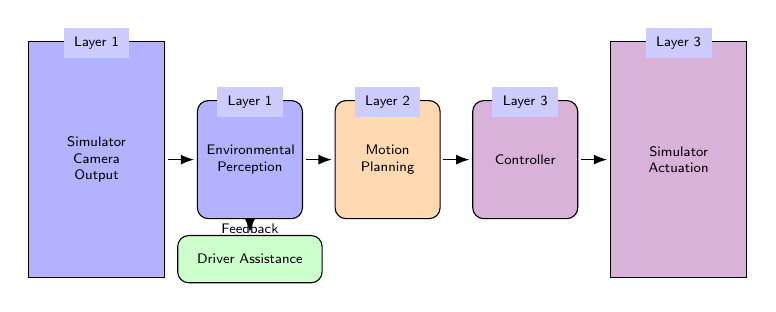
\begin{tikzpicture}[
        node distance=0.4cm, % Further reduced node distance
        block/.style={rectangle, draw, text width=1.1cm, align=center, font=\sffamily\tiny, minimum height=1.5cm, inner ysep=2pt}, % Smaller text width, font, height, padding
        long_block/.style={rectangle, draw, text width=1.5cm, align=center, font=\sffamily\tiny, minimum height=3cm, inner ysep=2pt}, % Smaller text width, font, height, padding
        feedback_block/.style={rectangle, rounded corners, draw, text width=1.6cm, align=center, font=\sffamily\tiny, fill=green!20, minimum height=0.6cm, inner ysep=2pt}, % Smaller text width, font, height, padding
        layer_box/.style={rectangle, fill=blue!20, text width=0.6cm, align=center, font=\sffamily\tiny, anchor=north, yshift=5pt}, % Smaller text width and yshift
        arrow/.style={->, >=Latex, thin, shorten >=1pt, shorten <=1pt} % Thin arrows, shortened slightly
    ]

    % Nodes
    \node[long_block, fill=blue!30] (simulator_output) {Simulator \\
    Camera \\ Output};
    \node[layer_box] at (simulator_output.north) {Layer 1};

    \node[block, rounded corners, fill=blue!30, right=of simulator_output] (environmental_perception) {Environmental Perception};
    \node[layer_box] at (environmental_perception.north) {Layer 1};
    \node[block, rounded corners, fill=orange!30, right=of environmental_perception] (motion_planning) {Motion Planning};
    \node[layer_box] at (motion_planning.north) {Layer 2};
    \node[block, rounded corners, fill=violet!30, right=of motion_planning] (controller) {Controller};
    \node[layer_box] at (controller.north) {Layer 3};

    \node[long_block, fill=violet!30, right=of controller] (simulator_actuation) {Simulator Actuation};
    \node[layer_box] at (simulator_actuation.north) {Layer 3};

    \node[feedback_block, below=of environmental_perception, yshift=0.2cm] (driver_assistance) {Driver Assistance};
 % Adjusted yshift
    \node[above=0mm of driver_assistance, font=\sffamily\tiny, anchor=south, yshift=-1mm] {Feedback};
 % Adjusted yshift


    % Arrows
    \draw[arrow] (simulator_output) -- (environmental_perception);
    \draw[arrow] (environmental_perception) -- (motion_planning);
    \draw[arrow] (motion_planning) -- (controller);
    \draw[arrow] (controller) -- (simulator_actuation);
    \draw[arrow] (environmental_perception.south) -- (driver_assistance.north);
    \end{tikzpicture}
    \caption{Proposed three-layer software architecture for the autonomous driving system.}      \label{fig:system_architecture}
\end{figure}

\subsection{Layer 1: Perception}
The perception layer is responsible for interpreting the vehicle's environment.
It uses a virtual RGB camera in CARLA as its primary sensor.
The raw image data is processed by the YOLOv8 object detection algorithm to identify and classify relevant objects, such as other vehicles and traffic signs.
In addition to providing data for the planning layer, this layer generates real-time visual feedback for the driver, including bounding boxes around detected objects, classification labels, and confidence scores, directly addressing our primary hypothesis.
\subsection{Layer 2: Planning}
The planning layer receives structured data from the perception layer and is responsible for generating safe and feasible trajectories.
It follows a hierarchical structure:
\begin{itemize}
    \item \textbf{Mission Planner:} Defines the high-level route using a predefined sequence of waypoints, each with a target velocity.
    \item \textbf{Behavioral Planner:} Uses a Finite State Machine (FSM) to make tactical decisions based on environmental context.
The FSM transitions between states like \texttt{FOLLOW\_LANE}, \texttt{DECELERATE\_TO\_STOP}, and \texttt{STAY\_STOPPED} in response to detected traffic signs (e.g., stop signs).
    \item \textbf{Local Planner:} Generates smooth, kinematically feasible, and collision-free paths to execute the behavioral planner's decisions.
It uses a Conformal Lattice Planner to create multiple candidate paths and selects the optimal one based on safety, comfort, and efficiency criteria.
\end{itemize}

\subsection{Layer 3: Control}
The control layer executes the trajectory generated by the local planner by sending precise commands to the vehicle's actuators in the CARLA simulator.
It is composed of two independent controllers based on the kinematic bicycle model:
\begin{itemize}
    \item \textbf{Longitudinal Control:} A Proportional-Integral-Derivative (PID) controller manages the vehicle's speed.
It calculates the error between the current speed and the target speed from the trajectory's velocity profile and applies throttle or brake commands to minimize this error.
The PID control law is given by:
    \begin{equation}
        u(t) = K_p e(t) + K_i \int_{0}^{t} e(\tau)d\tau + K_d\frac{de(t)}{dt}
    \end{equation}
    where $u(t)$ is the control signal, $e(t)$ is the velocity error, and $K_p, K_i, K_d$ are the proportional, integral, and derivative gains, respectively.
    \item \textbf{Lateral Control:} A Pure Pursuit controller manages steering. It identifies a target point on the reference path ahead of the vehicle (at a "lookahead distance") and calculates the steering angle required to navigate the vehicle along a circular arc to intercept that point.
The steering angle $\delta$ is calculated as:
    \begin{equation}
       \delta(t) = \arctan{\left(\frac{2L\sin{\alpha(t)}}{l_d}\right)}
    \end{equation}
    where $L$ is the vehicle's wheelbase, $\alpha(t)$ is the angle to the lookahead point, and $l_d$ is the lookahead distance, which is adapted based on the vehicle's speed.
\end{itemize}

\section{Implementation Details}
\label{sec:implementation}
The system was implemented using Python, leveraging the CARLA simulator (version 0.8.4) for the environment and vehicle dynamics.
The implementation follows the modular architecture described in Section \ref{sec:methodology}.
\subsection{Technical Environment}
A key technical challenge was the incompatibility between the CARLA simulator client, which requires Python 3.6, and modern deep learning libraries like PyTorch (for YOLOv8), which require Python 3.8+.
To overcome this, we designed a distributed client-server architecture (Figure \ref{fig:distributed_architecture_impl}).
%%% FIGURE 2: RECREATED WITH TIKZ FOR HIGH QUALITY AND ENGLISH LABELS (CORRECTED)
\begin{figure}[H]
    \centering
    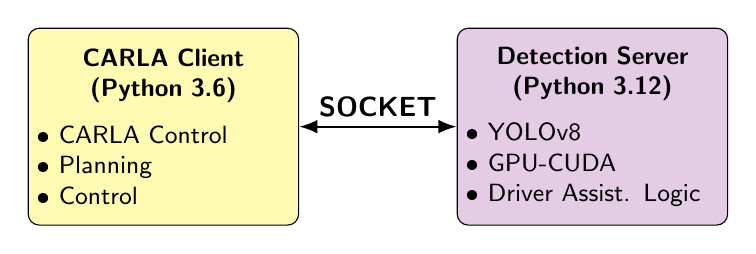
\begin{tikzpicture}[
        node distance=2cm,
        block/.style={rectangle, rounded corners, draw, text width=3.2cm, align=left, font=\sffamily\small, minimum height=2.5cm, inner ysep=5pt},
        client_block/.style={block, fill=yellow!30},
        server_block/.style={block, fill=violet!20},
        arrow/.style={<->, >=Latex, thick, font=\sffamily\bfseries}
    ]
    \node[client_block] (client) at (0,0) {\centering\textbf{CARLA Client (Python 3.6)}\par\vspace{2mm}\raggedright \textbullet~CARLA Control \\ \textbullet~Planning \\ \textbullet~Control};
    \node[server_block, right=of client] (server) {\centering\textbf{Detection Server (Python 3.12)}\par\vspace{2mm}\raggedright \textbullet~YOLOv8 \\ \textbullet~GPU-CUDA \\ \textbullet~Driver Assist. Logic};
    \draw[arrow] (client) -- (server) node[midway, above] {SOCKET};
    \end{tikzpicture}
    \caption{Distributed client-server architecture to overcome Python version incompatibility.}
    \label{fig:distributed_architecture_impl}
\end{figure}

\begin{itemize}
    \item \textbf{Client (Python 3.6):} Runs within the CARLA environment.
It is responsible for vehicle control, planning, and capturing camera frames.
It serializes and sends frames to the server via a TCP/IP socket.
    \item \textbf{Server (Python 3.12):} Runs in a separate Conda environment.
It receives frames, performs object detection using YOLOv8 with GPU acceleration (NVIDIA RTX 2060/4060), and sends the detection results (bounding boxes, classes, confidence scores) back to the client.
\end{itemize}
Communication was optimized using the MessagePack binary serialization protocol to minimize latency.
To ensure real-time performance and prevent the main control loop from being blocked by the detection process, an asynchronous, multi-threaded approach was implemented.
A producer thread captures frames and places them in a queue, while a consumer thread sends them to the detection server, ensuring the control loop remains responsive.
\subsection{Module Implementation}
\begin{itemize}
    \item \textbf{Perception Module:} The YOLOv8s (small) model was used, providing an excellent balance of speed and accuracy.
The model was pre-trained on the COCO dataset, which includes relevant classes like 'car' and 'stop sign'.
The detection server was configured to run on a GPU, achieving significant performance gains.
Visual feedback, including bounding boxes and persistent warnings, was rendered onto the camera feed using OpenCV on the client side.
    \item \textbf{Planning Module:} The behavioral planner was implemented as a simple FSM in the \texttt{behavioural\_planner.py} script.
It transitions between states based on vehicle speed and proximity to virtual fences representing stop signs, whose locations were pre-loaded from a configuration file.
The local planner, implemented in \texttt{local\_planner.py}, generates seven candidate paths using parametric spirals and selects the best collision-free path.
Collision checking is performed against static obstacles (parked cars) defined in a configuration file.
    \item \textbf{Control Module:} Both the PID longitudinal controller and the Pure Pursuit lateral controller were implemented within the \texttt{controller2d.py} script.
The PID gains ($K_p=0.5, K_i=0.3, K_d=0.13$) and the Pure Pursuit lookahead distance (2.0 meters, adapted with speed) were tuned empirically within the CARLA simulation to achieve stable and responsive vehicle behavior.
\end{itemize}

\subsection{Experimental Setup and Data Generation}
\label{sec:exp_setup}
Validation was performed in the CARLA simulator (version 0.8.4) on its publicly available \texttt{Town01} map.
Instead of using a pre-existing benchmark dataset, this study's "dataset" consists of quantitative metrics generated from a custom, predefined experimental route. This route was designed to test the system's core functionalities, including straight sections, a 90-degree turn, and a mandatory stop sign interaction.

Six independent simulation runs were conducted under three different weather conditions: \textit{Clear Noon}, \textit{Hard Rain Sunset}, and \textit{Hard Rain Noon}.
A comprehensive metrics collection system (\texttt{performance\_metrics.py}) was developed to log data on detection time, FPS, detection confidence, and vehicle dynamics.
The specific route configuration, simulation scripts, and all raw data generated and analyzed for this study are openly available, as detailed in the Data Availability Statement. This allows for full reproducibility of our experimental validation.

\section{Results and Discussion}
\label{sec:results}
The experimental validation yielded robust quantitative and qualitative data, allowing for a thorough assessment of the system's performance against the objectives and hypothesis.
The system successfully completed the entire predefined trajectory in all six simulation runs across all weather conditions, without any collisions.
\subsection{Perception System Performance}
The distributed architecture proved highly effective. The system achieved an average processing rate of \textbf{17.13 FPS}, significantly exceeding the target of 10 FPS.
The average detection time per frame was \textbf{59.4 ms}. A key finding was the system's robustness to adverse weather.
While the processing time was statistically significantly affected by weather conditions (ANOVA, p=0.025), with performance dropping to 14.41 FPS in heavy noon rain (likely due to the high computational cost of rendering heavy particle effects), the system remained well within real-time operational limits.

Crucially for our hypothesis, the confidence of the detections remained remarkably stable.
As shown in Table \ref{tab:results_by_weather}, the average confidence for stop sign detection was \textbf{0.738}, with a coefficient of variation of only \textbf{0.58\%} across all weather conditions.
An ANOVA test confirmed that there was no statistically significant difference in stop sign detection confidence between the weather conditions (p=0.651), demonstrating the system's reliability.
On the predefined experimental route, the system achieved a \textbf{100\% detection rate} for the target objects (all stop signs and vehicles) present in the trajectory.

\begin{table}[H]
\centering
\caption{Key performance metrics across different weather conditions.}
\label{tab:results_by_weather}
\resizebox{\columnwidth}{!}{%
\begin{tabular}{@{}lcccc@{}}
\toprule
\textbf{Metric} & \textbf{Clear Noon} & \textbf{Rain Sunset} & \textbf{Rain Noon} & \textbf{Average} \\ \midrule
Avg.
FPS & 17.74 & 19.23 & 14.41 & \textbf{17.13} \\
Avg.
Detection Time (s) & 0.0566 & 0.0521 & 0.0694 & \textbf{0.0594} \\
Avg. Stop Sign Conf.
& 0.734 & 0.743 & 0.737 & \textbf{0.738} \\ \bottomrule
\end{tabular}%
}
\end{table}

\subsection{Planning and Control Performance}
The planning and control modules performed flawlessly.
The behavioral planner's FSM correctly transitioned states upon approaching the stop sign in every run.
Figure \ref{fig:velocity_profile} shows a representative velocity profile, clearly illustrating the deceleration for the stop sign, the brief period of being stationary, and the subsequent re-acceleration.
\begin{figure}[H]
    \centering
    \includegraphics[width=0.7\columnwidth]{Figures/forward_speed.png}
    \caption{Vehicle's forward speed profile during a simulation run, showing the stop maneuver.}
    \label{fig:velocity_profile}
\end{figure}

The lateral control was also successful.
The vehicle maintained its lane on straight sections and executed the 90-degree turn smoothly.
The local planner successfully generated collision-free paths around the parked vehicle obstacle in all simulations.

\subsection{Discussion and Comparison with Related Work}
The results provide strong empirical validation for our hypothesis.
The system consistently demonstrated its ability to:
\begin{enumerate}
    \item \textbf{Detect traffic signs in real-time:} Achieved with an average of 17.13 FPS.
    \item \textbf{Provide reliable feedback:} Stop sign detection confidence remained high (0.738) and stable across adverse conditions, and visual feedback was generated in 100\% of cases.
    \item \textbf{Enable reliable driving:} The vehicle successfully used this information to perform a mandatory stop and completed all trajectories without incident.
\end{enumerate}

It is important to contextualize the 100\% detection rate. This is not a generalized accuracy metric (e.g., mAP) on a large-scale benchmark dataset, but rather a system validation metric specific to our controlled, predefined experimental route. This result confirms the system's ability to complete its intended task in a known environment, which was the objective of the study. This focus on system-level validation differentiates our work from studies that focus purely on perception-level optimization.

For instance, while our work focuses on the end-to-end integration of a complete autonomous pipeline, other studies have focused on optimizing the accuracy of the perception module itself. \citet{Wu_2022} and \citet{s23167145} propose architectural improvements to YOLOv4 and YOLOv7, respectively, to enhance the detection of small traffic signs, achieving high mAP scores on the challenging TT100K benchmark dataset. Our contribution is complementary: we demonstrate that a modern, off-the-shelf detector like YOLOv8 is sufficiently robust for real-time integration into a full Perception-Planning-Control loop, maintaining stable detection confidence even under adverse simulated weather.

One limitation observed was the occurrence of some false positive detections with high confidence (e.g., classifying parts of a car as a 'motorcycle').
This highlights a known challenge in deep learning models and suggests that for safety-critical applications, further model fine-tuning or supplementary validation logic would be necessary.
However, since the primary focus was on stop sign detection, which was highly reliable, this did not compromise the validation of our core hypothesis.

\section{Conclusion and Future Work}
\label{sec:conclusion}
This work successfully developed and validated an integrated driver assistance system based on YOLOv8 object detection within the CARLA simulator.
We empirically confirmed our hypothesis that such a system can provide reliable, real-time visual feedback of traffic signs, contributing to safer and more dependable driving.
The project yielded several key contributions, including a modular and functional three-layer autonomous driving architecture, a novel distributed processing solution to overcome software compatibility challenges, and a comprehensive experimental protocol for quantitative validation.
The results demonstrated that the system met or exceeded all predefined performance criteria.
It operated in real-time (avg. 17.13 FPS), achieved 100\% accuracy in detecting stop signs and vehicles on its path, and showed remarkable robustness in detection confidence across varied weather conditions.
The integrated planning and control systems enabled the vehicle to autonomously navigate its route and correctly respond to traffic regulations, completing all test runs without collision.

Despite these successes, the study has limitations, primarily its reliance on a simulated environment and its validation on a single, predefined route with a limited set of objects (stop signs and cars).
Future work should focus on bridging the gap between simulation and the real world.
A key direction is to enhance the communication architecture; migrating from TCP/IP sockets to an inter-process shared memory system could drastically reduce latency and increase throughput, enabling the integration of multiple sensors.
Further research should also expand the system's capabilities by training and validating the detection of a wider variety of traffic signs, pedestrians, and cyclists.
Finally, integrating data from complementary sensors, such as LiDAR and RADAR, would create a more robust perception system through sensor fusion, further improving reliability in all environmental conditions.
\section*{Declarations} \label{sec:Declarations}

\begin{contributions}
D.T.G. designed the study, performed the experiments, analyzed the data, and was the main writer of the manuscript. A.D.R.T.
supervised the research, provided critical feedback, and reviewed the manuscript. Both authors read and approved the final manuscript.
\end{contributions}

\begin{interests}
The authors declare that they have no competing interests.
\end{interests}

\begin{acknowledgements}
I express my deep gratitude to all who contributed significantly to this research.
To my advisor, Prof. Dr. Annabell Del Real Tamariz, for her rigorous scientific guidance and continuous dedication.
To the Universidade Estadual do Norte Fluminense Darcy Ribeiro (UENF) and the Laboratório de Ciências Matemáticas, especially the P5 Laboratory, for providing the academic support and computational resources essential for the experiments.
To my family, Carlos and Delma, and my fiancée, Maria, for their unconditional support and encouragement.
To my colleagues for enriching scientific discussions and to the researchers whose work provided the theoretical foundation for this investigation.
\end{acknowledgements}

\begin{funding}
This research was supported by a scientific initiation scholarship from the National Council for Scientific and Technological Development (CNPq) through the Institutional Program for Scientific Initiation Scholarships (PIBIC/CNPq).
\end{funding}

\begin{materials}
The complete source code, experimental data, configuration files, and automation scripts generated and analyzed during the current study are openly available in the following GitHub repository: \url{https://github.com/ARRETdaniel/CARLA_simulator_YOLO-openCV_realTime_objectDetection_for_autonomousVehicles/tree/main/CarlaSimulator/PythonClient/FinalProject}.
\end{materials}

\begin{filecontents*}{\jobname.bib}
@book{castro2009human,
  title={Human Factors of Visual and Cognitive Performance in Driving},
  editor={Castro, Candida},
  year={2009},
  publisher={CRC Press},
  address={Boca Raton, FL},
  isbn={978-1-4200-5530-6},
  doi={10.1201/9781420055313},
  url={http://www.crcpress.com}
}
@book{Vilanova2012,
  title={PID Control in the Third Millennium: Lessons Learned and New Approaches},
  editor={Vilanova, Ramon and Visioli, Antonio},
  year={2012},
  publisher={Springer},
  address={London},
  isbn={978-1-4471-2424-5},
  url={https://link.springer.com/book/10.1007/978-1-4471-2425-2},
  doi={10.1007/978-1-4471-2425-2}
}
@book{endsley2016designing,
  title={Designing for Situation Awareness: An Approach to User-Centered Design},
  author={Endsley, Mica R.},
  year={2016},
  doi={10.1201/b11371},
  edition={2},
  publisher={CRC Press},
  address={Boca Raton, FL},
  isbn={978-1-4200-6358-5},
  url = {https://doi.org/10.1201/b11371}
}
@article{kato2015open,
  title={An open approach to autonomous vehicles},
  author={Kato, Shinpei and Takeuchi, Eijiro and Ishiguro, Yoshio and Ninomiya, Yoshiki and Takeda, Kazuya and Hamada, Tsuyoshi},
  journal={IEEE Micro},
  volume={35},
  number={6},
  pages={60--68},
  year={2015},
  publisher={IEEE},
  url={https://ieeexplore.ieee.org/document/7368032},
  doi={10.1109/MM.2015.133}
}
@article{liu2020deep,
  title={Deep learning for generic object detection: A survey},
  author={Liu, Li and Ouyang, Wanli and Wang, Xiaogang and Fieguth, Paul and Chen, Jie and Liu, Xinwang and Pietikäinen, Matti},
  journal={International Journal of Computer Vision},
  volume={128},
  number={2},
  pages={261--318},
  year={2020},
  publisher={Springer},
  doi={10.1007/s11263-019-01247-4},
  url={https://link.springer.com/article/10.1007/s11263-019-01247-4}
}
@inproceedings{lin2017focal,
  title={Focal loss for dense object detection},
  author={Lin, Tsung-Yi and Goyal, Priya and Girshick, Ross and He, Kaiming and Dollár, Piotr},
  booktitle={Proceedings of the IEEE International Conference on Computer Vision},
  pages={2980--2988},
  year={2017},
  doi={10.1109/ICCV.2017.324},
  url={https://openaccess.thecvf.com/content_iccv_2017/html/Lin_Focal_Loss_for_ICCV_2017_paper.html}
}
@misc{carion2020end,
    title={End-to-End Object Detection with Transformers}, 
    author={Nicolas Carion and Francisco Massa and Gabriel Synnaeve and Nicolas Usunier and Alexander Kirillov and Sergey Zagoruyko},
    year={2020},
    eprint={2005.12872},
    archivePrefix={arXiv},
    primaryClass={cs.CV},
    url={https://arxiv.org/abs/2005.12872}
}
@misc{yaseen2024yolov8indepthexplorationinternal,
    title={What is YOLOv8: An In-Depth Exploration of the Internal Features of the Next-Generation Object Detector}, 
    author={Muhammad Yaseen},
    year={2024},
    eprint={2408.15857},
    archivePrefix={arXiv},
    primaryClass={cs.CV},
    url={https://arxiv.org/abs/2408.15857}
}
@book{kopetz2011real,
  title={Real-Time Systems: Design Principles for Distributed Embedded Applications},
  author={Kopetz, Hermann},
  year={2011},
  publisher={Springer},
  edition={2},
  address={New York},
  isbn={978-1-4419-8236-0},
  doi={10.1007/978-1-4419-8237-7},
  url={https://doi.org/10.1007/978-1-4419-8237-7}
}
@misc{iordache2021smart,
    title={Smart Pointers and Shared Memory Synchronisation for Efficient Inter-process Communication in ROS on an Autonomous Vehicle},
    author={Costin Iordache and Stephen M. Fendyke and Mike J. Jones and Robert A. Buckley},
    year={2021},
    eprint={2108.07085},
    archivePrefix={arXiv},
    primaryClass={cs.RO},
    doi={10.48550/arXiv.2108.07085},
    url={https://arxiv.org/abs/2108.07085}
}
@article{rosique2019systematic,
    author = {Rosique, Francisca and Navarro, Pedro J. and Fernández, Carlos and Padilla, Antonio},
    title = {A Systematic Review of Perception System and Simulators for Autonomous Vehicles Research},
    journal = {Sensors},
    volume = {19},
    year = {2019},
    number = {3},
    article-number = {648},
    url = {https://www.mdpi.com/1424-8220/19/3/648},
    doi = {10.3390/s19030648}
}
@book{lavalle2006planning,
  title={Planning Algorithms}, 
  author={LaValle, Steven M},
  year={2006},
  url = {https://doi.org/10.1017/CBO9780511546877},
  publisher={Cambridge University Press}
}
@inproceedings{wei2014behavioral,
  title={A behavioral planning framework for autonomous driving},
  author={Wei, Junqing and Snider, Jarrod M and Gu, Tianyu and Dolan, John M and Litkouhi, Bakhtiar},
  booktitle={2014 IEEE Intelligent Vehicles Symposium Proceedings},
  pages={458--464},
  year={2014},
  organization={IEEE},
  url={https://ieeexplore.ieee.org/document/6856582},
  doi={10.1109/IVS.2014.6856582}
}
@book{sutton1998reinforcement,
  title={Reinforcement learning: An introduction},
  author={Sutton, Richard S. and Barto, Andrew G.},
  year={1998},
  publisher={MIT Press},
  address={Cambridge},
  edition={2},
  isbn={9780262193986},
  url={https://web.stanford.edu/class/psych209/Readings/SuttonBartoIPRLBook2ndEd.pdf}
}
@misc{wang2024yolov10realtimeendtoendobject,
    title={YOLOv10: Real-Time End-to-End Object Detection}, 
    author={Ao Wang and Hui Chen and Lihao Liu and Kai Chen and Zijia Lin and Jungong Han and Guiguang Ding},
    year={2024},
    eprint={2405.14458},
    archivePrefix={arXiv},
    primaryClass={cs.CV},
    url={https://arxiv.org/abs/2405.14458}
}
@article{wang_yolov1_to_yolov10,
  author={Wang, Chien-Yao and Liao, Hong-Yuan Mark},
  title={{YOLOv1 to YOLOv10: The Fastest and Most Accurate Real-Time Object Detection Systems}},
  journal={arXiv preprint arXiv:2408.09332},
  year={2024},
  url={https://arxiv.org/abs/2408.09332}
}
@misc{wu_physical_adversarial_attack,
  author={Wu, T. and others},
  title={{Physical Adversarial Attack on Vehicle Detector in the Carla Simulator}},
  journal={arXiv preprint arXiv:2007.16118},
  year={2020},
  url={http://arxiv.org/abs/2007.16118}
}
@misc{redmon2018yolov3incrementalimprovement,
    title={YOLOv3: An Incremental Improvement}, 
    author={Joseph Redmon and Ali Farhadi},
    year={2018},
    eprint={1804.02767},
    archivePrefix={arXiv},
    primaryClass={cs.CV},
    url={https://arxiv.org/abs/1804.02767}
}
@misc{redmon2016lookonceunifiedrealtime,
    title={You Only Look Once: Unified, Real-Time Object Detection}, 
    author={Joseph Redmon and Santosh Divvala and Ross Girshick and Ali Farhadi},
    year={2016},
    eprint={1506.02640},
    archivePrefix={arXiv},
    primaryClass={cs.CV},
    url={https://arxiv.org/abs/1506.02640}
}
@article{bochkovskiy2020yolov4optimalspeedaccuracy,
  author={Alexey Bochkovskiy and Chien-Yao Wang and Hong-Yuan Mark Liao},
  title={YOLOv4: Optimal Speed and Accuracy of Object Detection},
  journal={arXiv preprint arXiv:2004.10934},
  year={2020},
  url={https://arxiv.org/abs/2004.10934}
}
@article{Wu_2022,
    doi = {10.1088/1742-6596/2258/1/012009},
    url = {https://dx.doi.org/10.1088/1742-6596/2258/1/012009},
    year = {2022},
    month = {apr},
    publisher = {IOP Publishing},
    volume = {2258},
    number = {1},
    pages = {012009},
    author = {Xiru Wu and Haozhe Cao},
    title = {Traffic Sign Detection Algorithm Based On Improved YOLOv4},
    journal = {Journal of Physics: Conference Series}
}
@incollection{wachenfeld_release_autonomous_vehicles,
  author={Wachenfeld, W. and Winner, H.},
  title={{The Release of Autonomous Vehicles}},
  booktitle={Autonomous Driving: Technical, Legal and Social Aspects},
  editor={Maurer, M. and others},
  pages={425--449},
  year={2016},
  publisher={Springer},
  address={Berlin, Heidelberg},
  doi={10.1007/978-3-662-48847-8\_21}
}
@article{ahire2024simulating,
  author={Ahire, Prashant and Naidu, SMM and Varpe, Sandeep and Nadarge, Sakshi and Patil, Anushree},
  title={Simulating Vehicle Driving Using CARLA},
  journal={Journal of Electrical Systems},
  volume={20},
  number={10s},
  pages={44--52},
  year={2024},
  publisher={Engineering and Scientific Research Groups},
  url={https://journal.esrgroups.org/jes/article/view/5022}
}
@article{janai_computer_vision_av,
    author = {Janai, Joel and Güney, Fatma and Behl, Aseem and Geiger, Andreas},
    title = {Computer Vision for Autonomous Vehicles: Problems, Datasets and State of the Art},
    year = {2020},
    publisher = {Now Publishers Inc.},
    volume = {12},
    number = {1–3},
    journal = {Foundations and Trends in Computer Graphics and Vision},
    pages = {1–308},
    doi={10.1561/0600000079}
}
@misc{lanctot_passenger_economy,
  author={Roger Lanctot},
  title={{Accelerating the Future: The Economic Impact of the Emerging Passenger Economy}},
  year={2017},
  publisher={Strategy Analytics},
  url={https://www.intel.com/content/dam/www/public/us/en/documents/pdf/passenger-economy-report-autonomous-driving.pdf}
}
@misc{nhtsa_crash_causation,
  author={{National Highway Traffic Safety Administration}},
  title={Critical Reasons for Crashes Investigated in the National Motor Vehicle Crash Causation Survey: DOT HS 812 506 A Brief Statistical Summary},
  year={2018},
  url={https://crashstats.nhtsa.dot.gov/Api/Public/Publication/812506}
}
@article{okpono2024advanced,
  author={Okpono, Joseph and Asedegbega, Jerome and Ogieva, Mathew and Sanyaolu, Temitope Oluwafunmike},
  title={Advanced driver assistance systems road accident data insights: Uncovering trends and risk factors},
  journal={The International Journal of Engineering Research},
  year={2024},
  volume={11},
  number={9},
  pages={a141--a152},
  doi={10.5281/zenodo.13817419},
  url={https://tijer.org/tijer/papers/TIJER2409017.pdf}
}
@misc{eu_safer_roads,
  author={{European Commission, Directorate-General for Mobility and Transport}},
  title={{Safer roads for all: EU Road Safety Policy Framework 2021-2030}},
  year={2021},
  url={https://road-safety.transport.ec.europa.eu/system/files/2021-07/safer_roads4all.pdf}
}
@techreport{snider2009automatic,
  title={Automatic Steering Methods for Autonomous Automobile Path Tracking},
  author={Snider, Jarrod M.},
  institution={Robotics Institute, Carnegie Mellon University},
  number={CMU-RI-TR-09-08},
  year={2009},
  url={https://www.ri.cmu.edu/pub_files/2009/2/Automatic_Steering_Methods_for_Autonomous_Automobile_Path_Tracking.pdf}
}
@inproceedings{dosovitskiy2017carla,
  author={Dosovitskiy, Alexey and Ros, German and Codevilla, Felipe and Lopez, Antonio and Koltun, Vladlen},
  title={{CARLA: An open urban driving simulator}},
  booktitle={Proceedings of the Conference on Robot Learning},
  pages={1--16},
  year={2017},
  organization={PMLR},
  url={https://proceedings.mlr.press/v78/dosovitskiy17a.html}
}
@article{aplicacao2,
    title = {Autonomous Vehicles and Intelligent Automation: Applications, Challenges, and Opportunities},
    author  = {Gourav Bathla and Kishor Bhadane and Rahul Kumar Singh},
    journal = {Mobile Information Systems},
    year = {2022},
    publisher = {Hindawi},
    doi = {10.1155/2022/7632892}
}
@article{sensors-yet,
  title={Level-5 autonomous driving—are we there yet?
 A review of research literature},
  author={Khan, Manzoor Ahmed and Sayed, Hesham El and Malik, Sumbal and Zia, Talha and Khan, Jalal and Alkaabi, Najla and Ignatious, Henry},
  journal={ACM Computing Surveys},
  year={2022},
  publisher={ACM},
  doi={10.1145/3485767}
}
@article{SAE,
    title = {Taxonomy and Definitions for Terms Related to Driving Automation Systems for On-Road Motor Vehicles},
    author={{SAE International}},
    journal = {SAE J3016\_202104},
    year = {2021},
    publisher = {SAE International},
    doi = {10.4271/J3016\_202104}
}
@misc{Center_of_Automotive_Management2022,
  author={Bratzel, Stefan and {Center of Automotive Management}},
  title={{Die Zukunft der Mobilität – Die Zukunftstrends in den Bereichen Elektromobilität, Connected Car und Mobilitätsdienstleistungen}},
  year={2022},
  url={https://www.bnpparibas.de/de/studie-zu-aktuellem-umbruch-der-mobilitaetsbranche/}
}
@article{review-auto,
    title = {A Review on Autonomous Vehicles: Progress, Methods and Challenges},
    author  = {Darsh Parekh and Nishi Poddar and Manisha Chahal},
    year = {2022},
    journal = {Electronics},
    publisher = {MDPI},
    volume = {11},
    number = {14},
    pages = {2162},
    doi = {10.3390/electronics11142162}
}
@misc{intro-pm,
    title = {Global fleet of autonomous vehicles may emit more carbon than Argentina},
    author = {Dreibelbis, Emily},
    howpublished = {PCMag},
    year = {2023},
    url = {https://www.pcmag.com/news/global-fleet-of-autonomous-vehicles-may-emit-more-carbon-than-argentina}
}
@article{mundobrasil,
  author={Othman, Kareem},
  title={Multidimension Analysis of Autonomous Vehicles: The Future of Mobility},
  journal={Civil Engineering Journal},
  year={2021},
  volume={7},
  number={7},
  pages={71--93},
  doi={10.28991/CEJ-SP2021-07-06}
}
@inproceedings{sebo2024impact,
  title={{Impact of electric vehicle market growth on automotive industry transformation: trends, potentials, and challenges analysis}},
  author={Sebo, Damir},
  booktitle={Economic and Social Development (Book of Proceedings), 106th International Scientific Conference on Economic and Social Development},
  year={2024}
}
@article{conge,
    author = {Neufville, Roxanne and Abdalla, Hassan and Abbas, Ali},
    title = {Potential of Connected Fully Autonomous Vehicles in Reducing Congestion and Associated Carbon Emissions},
    journal = {Sustainability},
    volume = {14},
    year = {2022},
    number = {11},
    article-number = {6910},
    doi = {10.3390/su14116910}
}

@misc{4cenarios_ocidental,
  title={Quatro Cenários para os Veículos Autônomos no Mundo Ocidental},
  author={Cíntia Alvim Lage},
  howpublished = {Repositório Institucional da UnB},
  year={2019},
  url={https://repositorio.unb.br/handle/10482/38474}
}
@misc{KPMG,
  author={{KPMG International}},
  title={{2020 Autonomous Vehicles Readiness Index}},
  year={2020},
  url={https://assets.kpmg.com/content/dam/kpmg/xx/pdf/2020/07/2020-autonomous-vehicles-readiness-index.pdf}
}
@misc{mercedes3,
  title={{Mercedes-Benz erhält als weltweit erstes Automobilunternehmen Zertifizierung für SAE Level 3-System für US-Markt}},
  author={Mitropoulos, Alexandros},
  year={2023},
  publisher={Mercedes-Benz Group AG},
  url={https://group-media.mercedes-benz.com/marsMediaSite/de/instance/ko.xhtml?oid=55116818}
}
@misc{Houser2023-dn,
  title={{Mercedes-Benz} wins race to bring Level 3 autonomous cars to {US}},
  author={Houser, Kristin},
  howpublished={Freethink Media},
  year={2023},
  url={https://www.freethink.com/hard-tech/drive-pilot}
}
@mastersthesis{sanchez_speed_sign_detection,
  author={Sánchez Juanola, Martí},
  title={{Speed Traffic Sign Detection on the CARLA Simulator Using YOLO}},
  school={Universitat Pompeu Fabra},
  year={2019},
  url={http://hdl.handle.net/10230/42548}
}
@misc{andrade_object_detection_distance,
  author={Andrade, Guilherme Guy de},
  title={{Uma Proposta para Detecção de Objetos e Estimação de Distância em um Simulador de Veículos Autônomos}},
  year={2022},
  howpublished={Trabalho de Conclusão de Curso (Graduação) – Universidade de Brasília},
  url={https://github.com/guilherme1guy/carla_darknet_integration}
}
@article{s23167145,
    author = {Li, Songjiang and Wang, Shilong and Wang, Peng},
    title = {A Small Object Detection Algorithm for Traffic Signs Based on Improved YOLOv7},
    journal = {Sensors},
    volume = {23},
    year = {2023},
    number = {16},
    article-number = {7145},
    doi = {10.3390/s23167145}
}
@misc{University_of_Toronto2018-fe,
  title={{Introduction to Self-Driving Cars}},
  author={{University of Toronto}},
  publisher={Coursera Inc},
  year={2018},
  note={Part of the Self-Driving Cars Specialization},
  url={https://www.coursera.org/learn/intro-self-driving-cars?specialization=self-driving-cars}
}
@misc{University_of_Toronto2018-mp,
  title={{Motion Planning for Self-Driving Cars}},
  author={{University of Toronto}},
  publisher={Coursera Inc},
  year={2018},
  note={Part of the Self-Driving Cars Specialization},
  url={https://www.coursera.org/learn/motion-planning-self-driving-cars}
}
@article{paden2016survey,
  author={Paden, Brian and Čáp, Michal and Yong, Sze Zheng and Yershov, Dmitry and Frazzoli, Emilio},
  title={A survey of motion planning and control techniques for self-driving urban vehicles},
  journal={IEEE Transactions on Intelligent Vehicles},
  year={2016},
  volume={1},
  number={1},
  pages={33--55},
  doi={10.1109/TIV.2016.2578706}
}
@article{jacobson2020vehicle,
  title={Vehicle dynamics COMPENDIUM},
  author={Jacobson, Bengt},
  journal={Chalmers University of Technology},
  year={2020},
  url={https://research.chalmers.se/en/publication/520229}
}
@article{jacobson2016vehicle,
  title={Vehicle dynamics},
  author={Jacobson, Bengt},
  journal={Chalmers University of Technology},
  year={2016},
  url={https://publications.lib.chalmers.se/records/fulltext/244369/244369.pdf}
}
@book{francis2016models,
    author="Francis, Bruce A. and Maggiore, Manfredi",
    title="Models of Mobile Robots in the Plane",
    bookTitle="Flocking and Rendezvous in Distributed Robotics",
    year="2016",
    publisher="Springer International Publishing",
    doi="10.1007/978-3-319-24729-8\_2"
}
@mastersthesis{bussemaker2014sensing,
  title={Sensing requirements for an automated vehicle for highway and rural environments},
  author={Bussemaker, KJ},
  school={Delft University of Technology},
  year={2014},
  url={https://resolver.tudelft.nl/uuid:2ae44ea2-e5e9-455c-8481-8284f8494e4e}
}
@article{pivtoraiko2009differentially,
  title={Differentially constrained mobile robot motion planning in state lattices},
  author={Pivtoraiko, Mihail and Knepper, Ross A and Kelly, Alonzo},
  journal={Journal of Field Robotics},
  volume={26},
  number={3},
  pages={308--333},
  year={2009},
  doi={10.1002/rob.20285}
}
@article{kim2023challenges,
  author          = {Kim, Taesoo and Jeon, Hyeonjae and Lim, Yongseob},
  title           = {Challenges of YOLO Series for Object Detection in Extremely Heavy Rain: CALRA Simulator based Synthetic Evaluation Data set},
  journal         = {arXiv preprint arXiv:2312.07976},
  year            = {2023},
  url             = {https://arxiv.org/abs/2312.07976}
}
\end{filecontents*}

\bibliographystyle{apalike-sol}
\bibliography{\jobname}


%%%%%%%%%%%%%%%%%%%%%%%%%%%%%%%%%%%%%%%%%%%%%%%%%%%%%%%%%%%%%%%%%%%%%%%%%%%%%%%%
% JBCS Submission - Reviewer Commitment Information
% As per submission guidelines.
%%%%%%%%%%%%%%%%%%%%%%%%%%%%%%%%%%%%%%%%%%%%%%%%%%%%%%%%%%%%%%%%%%%%%%%%%%%%%%%%
\begin{comment}
Reviewer Commitment Information:

Reviewer’s full name: Annabell Del Real Tamariz
Area of expertise: Data Science, Autonomous Vehicles, Artificial Intelligence
Institutional Email Address: annabell@uenf.br
Highest Academic Degree: Ph.D.
\end{comment}

\end{document}